% Use only LaTeX2e, calling the article.cls class and 12-point type.

\documentclass[12pt]{article}

\usepackage{graphicx}

\newcommand\aap{{A\&A}}% 
         % Astronomy and Astrophysics 
\newcommand\aaps{{A\&AS}}% 
         % Astronomy and Astrophysics, Supplement 
\newcommand\aj{{AJ}}% 
         % Astronomical Journal 
\newcommand\araa{{ARA\&A}}% 
         % Annual Review of Astron and Astrophys 
\newcommand\apj{{ApJ}}% 
         % Astrophysical Journal 
\newcommand\apjl{{ApJ}}% 
         % Astrophysical Journal, Letters 
\newcommand\apjs{{ApJS}}% 
         % Astrophysical Journal, Supplement 
\newcommand\mnras{{MNRAS}}% 
         % Monthly Notices of the RAS 
\newcommand\nat{{Nature}}% 
         % Nature 
\newcommand\pasp{{PASP}}% 
         % Publications of the ASP 
\newcommand{\cubecm}{\ifmmode{{\rm cm^{-3}}}\else{cm$^{-3}$}\fi}
\newcommand{\lsim}{\lower0.3em\hbox{$\,\buildrel <\over\sim\,$}}
\newcommand{\gsim}{\lower0.3em\hbox{$\,\buildrel >\over\sim\,$}}
\newcommand{\kms}{\ifmmode{{\rm km~s^{-1}}}\else{km s$^{-1}$}\fi}
\newcommand{\hh}{H$_2$}
\newcommand{\Ms}{\ifmmode{M_\odot}\else{$M_\odot$}\fi}
\newcommand\tento[1]{$10^{#1}$}
\newcommand{\tvir}{\ifmmode{T_{\rm{vir}}}\else{$T_{\rm{vir}}$}\fi}

% Users of the {thebibliography} environment or BibTeX should use the
% scicite.sty package, downloadable from *Science* at
% www.sciencemag.org/about/authors/prep/TeX_help/ .
% This package should properly format in-text
% reference calls and reference-list numbers.

%% We will uncomment this later
\usepackage{scicite}
\bibliographystyle{Science}

% Use times if you have the font installed; otherwise, comment out the
% following line.

\usepackage{times}

% The preamble here sets up a lot of new/revised commands and
% environments.  It's annoying, but please do *not* try to strip these
% out into a separate .sty file (which could lead to the loss of some
% information when we convert the file to other formats).  Instead, keep
% them in the preamble of your main LaTeX source file.


% The following parameters seem to provide a reasonable page setup.

\topmargin 0.0cm
\oddsidemargin 0.2cm
\textwidth 16cm 
\textheight 21cm
\footskip 1.0cm


%The next command sets up an environment for the abstract to your paper.

\newenvironment{sciabstract}{%
\begin{quote} \bf}
{\end{quote}}


% If your reference list includes text notes as well as references,
% include the following line; otherwise, comment it out.

\renewcommand\refname{References and Notes}

% The following lines set up an environment for the last note in the
% reference list, which commonly includes acknowledgments of funding,
% help, etc.  It's intended for users of BibTeX or the {thebibliography}
% environment.  Users who are hand-coding their references at the end
% using a list environment such as {enumerate} can simply add another
% item at the end, and it will be numbered automatically.

\newcounter{lastnote}
\newenvironment{scilastnote}{%
\setcounter{lastnote}{\value{enumiv}}%
\addtocounter{lastnote}{+1}%
\begin{list}%
{\arabic{lastnote}.}
{\setlength{\leftmargin}{.22in}}
{\setlength{\labelsep}{.5em}}}
{\end{list}}


% Include your paper's title here

\title{The Birth of a Galaxy: Population III Metal Enrichment and
  Population II Stellar Populations}


% Place the author information here.  Please hand-code the contact
% information and notecalls; do *not* use \footnote commands.  Let the
% author contact information appear immediately below the author names
% as shown.  We would also prefer that you don't change the type-size
% settings shown here.

\author
{John H.~Wise,$^{1,2\ast}$ Michael L.~Norman,$^{3}$ Tom Abel$^{4}$,
Matthew J.~Turk$^{3}$\\
\\
\normalsize{$^{1}$Department of Astrophysical Sciences, Princeton
University,}\\
\normalsize{Peyton Hall, Ivy Lane, Princeton, NJ 08544}\\
\normalsize{$^{2}$Hubble Fellow}\\
\normalsize{$^{3}$Center for Astrophysics and Space Sciences,}\\
\normalsize{University of California at San Diego, La Jolla, CA 92093}\\
\normalsize{$^{4}$Kavli Institute for Particle Astrophysics and
  Cosmology, }\\
\normalsize{Stanford University, Menlo Park, CA 94025}\\
\\
\normalsize{$^\ast$To whom correspondence should be addressed; E-mail:
jwise@astro.princeton.edu}
}

% Include the date command, but leave its argument blank.

\date{}



%%%%%%%%%%%%%%%%% END OF PREAMBLE %%%%%%%%%%%%%%%%



\begin{document} 

% Double-space the manuscript.

\baselineskip24pt

% Make the title.

\maketitle 

% Place your abstract within the special {sciabstract} environment.

\begin{sciabstract}
  Supernova explosions from the first stars in the universe, which are
  predicted to be very massive, chemically enriched the intergalactic
  medium, originally a primordial mix of hydrogen and helium.  A
  fraction of these metals propagate into star-forming regions,
  providing more efficient cooling mechanisms and, in turn, increasing
  gaseous fragmentation in the first stellar clusters.  Here, we
  report on the birth of two high-redshift dwarf galaxies in a
  cosmological radiation hydrodynamics simulation.  We find that only
  one supernova is sufficient to enrich the nearby star-forming gas
  with a floor of 1/1,000 of the solar metallicity ratio, preventing
  any further metal-free star formation within 10 kpc of the past
  explosion.  We follow the entire star formation history of these
  galaxies, providing robust models to interpret the stellar
  populations of nearby dwarf galaxies and future observations of
  high-redshift dwarf galaxies.
\end{sciabstract}

% In setting up this template for *Science* papers, we've used both
% the \section* command and the \paragraph* command for topical
% divisions.  Which you use will of course depend on the type of paper
% you're writing.  Review Articles tend to have displayed headings, for
% which \section* is more appropriate; Research Articles, when they have
% formal topical divisions at all, tend to signal them with bold text
% that runs into the paragraph, for which \paragraph* is the right
% choice.  Either way, use the asterisk (*) modifier, as shown, to
% suppress numbering.

\section*{Motivation}

The first (Pop III) stars are metal-free and have a large
characteristic mass and suppressed fragmentation in its protostellar
collapse \cite{ABN02, Bromm02_P3, Yoshida03, OShea07a}.  A fraction of
these stars enrich the surrounding intergalactic medium (IGM) when
they go supernova, which can happen in stars $\lsim 40~\Ms$ in Type II
supernovae (SNe) or in stars roughly between 140 \Ms~and 260 \Ms~in
pair-instability SNe (PISNe; \cite{2002ApJ...567..532H}).  The host
halo and the neighboring halos are then enriched with this ejecta.
There exists a critical metallicity that is $\sim 10^{-6} Z_\odot$ if
dust cooling is efficient \cite{Omukai05, Schneider06_Frag, clark08}
and $\sim 10^{-3.5} Z_\odot$ otherwise \cite{Bromm01,
  2009ApJ...691..441S}, where the gas can cool rapidly, lowering its
Jeans mass.  An intermediate characteristic mass of $\sim10~\Ms$ can
be occur if the gas cooling is suppressed to the cosmic microwave
background (CMB) temperature \cite{Larson98, Tumlinson07_IMF,
  2009ApJ...691..441S}.  The resulting Population II star cluster will
thus have a lower characteristic stellar mass than its metal-free
progenitors.  These first stellar clusters may be connected to stars
in the Milky Way halo and nearby dwarf spheroidal (dSph) galaxies,
both with a metallicity floor of [Z/H] = --4 \cite{Beers05,
  Tafelmeyer10, Frebel10_Obs}.

The transition from Pop III to Pop II star formation (SF) is solely
dependent on the propagation of metals from the SNe remnants into
future sites of SF.  Their flows are complex because of the
interactions between the SN blastwave, cosmological accretion and halo
mergers, and nearby stellar feedback.  In minihalos ($M \sim
10^6~\Ms$), radiation from a massive Pop III star can drive a 30
\kms~shock, which is 10 times greater than the escape velocity of the
halo, and leaves behind a warm ($3 \times 10^4$ K) and diffuse (0.5
\cubecm) medium \cite{Kitayama04, Whalen04, Abel07}.  This aids in the
expansion of the blastwave because it delays the transition to the
Sedov-Taylor and snowplow phases.  In PISNe, approximately half of the
metals stay in the IGM with a metal bubble size of a few kpc
\cite{Wise08_Gal, Greif10}.  The blastwave may induce SF in nearby
halos through the compression of the gas \cite{Ferrara98}, and
timescales for metal mixing into the dense gas are many dynamical
times \cite{Cen08} for shock velocities $\lsim100~\kms$.

Numerical simulations are useful to detangle and study these
complexities and the transition from Pop III to II stars.  In this
Report, we present the simulations that include both types of SF, and
their radiative and mechanical feedback.  The methods used here
incorporate and link together recent results from metal-enriched and
metal-free star formation, the critical metallicity, and
pair-instability supernovae.  This is the first simulation that can
resolve star-forming minihalos while following the transition to Pop
II star formation in the first galaxies.

\section*{Results}
\label{sec:results}

Here we present the gaseous and stellar evolution of two selected
halos in the simulation: one that has an early mass buildup but no
major mergers after $z=12$, and one that experiences a series of major
mergers between $z=10$ and $z=7$.  We name the halos ``quiet'' and
``intense'', respectively.  

% We start with the mass accretion history and enrichment of the
% halos.  We then compare the nature of the stellar populations in
% these halos.

We illustrate the state of the simulation at $z=7$ in Figure
\ref{fig:projections} with density weighted projections of gas
density, temperature, and metallicity, showing the entire box and
focusing on the two halos of interest.  Radiative and mechanical
feedback create a multi-phase medium inside these halos, which are
embedded in a warm and ionized IGM.

\subsection*{Mass evolution}
\label{sec:halo}

%\li Describe the evolution of the baryon fraction and metallicity from
%PISN and Type II SNe metals in the two halos.

Figure \ref{fig:evo}a shows the total, metal-enriched stellar, and gas
mass history of the most massive progenitors of both halos.  The quiet
halo undergoes a series of major mergers at $z > 12$, growing by a
factor of 30 to $2.5 \times 10^7 \Ms$ within 150 Myr.  Afterwards it
only grows by a factor of 3 by $z=7$ mainly through smooth accretion
from the filaments and IGM.  It is the most massive halo in the
simulation between redshifts 13 and 10.  At the same time, the intense
halo has a mass $M = 3 \times 10^6 \Ms$, but it is contained in a
biased region on a comoving scale of 50 kpc with $\sim25$ halos with
$M \sim 10^6 \Ms$.  After $z=10$, these halos hierarchically merge to
form a $10^9 \Ms$ halo at $z=7$ with two major mergers at redshifts 10
and 7.9, seen in the rapid increases in total mass in Figure
\ref{fig:evo}a.  The merger history of the two halos are not atypical
as dark matter halos can experience both quiescent and vigorous mass
accretion rates in their buildup.

Both halos start forming Pop II stars when $M = 10^7 \Ms$.  This is
consistent with the filtering mass $M_f$ of high-redshift halos when
it accretes mainly from a pre-heated IGM \cite{gnedin98, gnedin00,
  Wise08_Gal}.  Afterwards these halos can cool efficiently through
\hh~cooling, sustaining constant and sometimes bursty SF.  The latter
characteristics are equated with the definition of a galaxy.  The
quiet halo forms $10^5 \Ms$ of stars by $z=9$.  This initial starburst
photo-evaporates the majority of its molecular clouds, in addition to
heating and ionizing the surrounding IGM out to a radius of 10--15 kpc
at $z=9$.  These respectively reduce the in-situ and external cold gas
supply that could feed future SF.

The gas fractions of both halos decrease from 0.15 to 0.08 by outflows
driven by ionization fronts and blastwaves in their initial
starbursts.  The quiet halo never recovers to the cosmic fraction
$\Omega_b/\Omega_M$ for the following reason.  The lack of major
mergers of halos above the filtering mass leads to a small gas
fraction because halos with $M < M_f$ are likely photo-evaporated,
hosting diffuse warm gas reservoirs instead of cold dense cores.
After $z=10$, the halo mainly accretes warm diffuse gas from the
filaments and IGM.  In contrast, the intense halo grows from major
mergers of halos with $M > M_f$.  The progenitor halos involved in the
major mergers are able to host molecular clouds and have, in general,
higher gas fractions.  Between $z=10$ and $z=8$, the gas fraction
increases from 0.07 to 0.12 until it jumps to 0.14 when a gas-rich
major merger occurs.  The stellar mass accordingly increases with the
ample supply of gas during this period.  The gas fraction then
decreases by 0.01 when galactic outflows are generated from the
starburst associated with this major merger.

\subsection*{Metallicity evolution}
\label{sec:zevo}

The evolution of the stellar and gas metallicity of both halos are
illustrated in Figure \ref{fig:evo}b.  PISNe from Pop III stars enrich
the nearby IGM out to a radius of 10 kpc and provides a metallicity
floor of $[Z_3/H] \sim -3$.  The metallicity from Pop II SNe initially
enrich the ISM of both halos to an average $[\bar{Z}_2/H]$ between
--3.5 and --3.  

\textit{Quiet halo}.--- Afterwards an equilbrium of $[\bar{Z}_2/H]
\sim -2.5$ is established between metal-rich outflows and metal-poor
inflows.  Galactic outflows are directed in the polar directions of
the gas disk, keeping the adjacent filaments metal-poor.  These
features and a well-mixed ISM (cf.~\cite{Wise08_Gal, Greif10}) are
apparent in the metallicity projections in Figure
\ref{fig:projections}.  The average stellar metallicity is within 0.5
dex of $[\bar{Z}_2/H]$.

\textit{Intense halo}.--- The first few Pop II star clusters have
$[Z/H]$ between --1 and --2 and dominate the average stellar
metallicity at $z > 8$.  Afterwards the metallicity increases by a
factor of 30 to $[\bar{Z}_2/H] = -1.5$ through self-enrichment from a
starburst.  Because this halo is located in a large-scale overdensity,
most of the ejecta falls back into the halo after reaching distances
up to 20 comoving kpc, in turn keeping the halo gas metallicity high
because the inflows are relatively metal-rich themselves.  After the
$z \sim 8$ starburst, the average stellar metallicity follows the
average gas metallicity within 0.1 dex.

\subsection*{Population III star formation history}

\textit{Quiet halo}.--- The most massive progenitor interestingly
never hosts a Pop III star.  Instead a nearby halo forms a Pop III
star, which (randomly) produces a PISNe at $z=16$.  The blastwave
overruns the most massive progenitor, and the dense core survives this
event and is enriched by this PISN, triggering the transition to Pop
II SF.  Other progenitors host three Pop III stars, forming at $z =
15.4, 14.2, 13.8$, with the latter producing a PISN.  Metal enrichment
from these two PISNe and Pop II SF quench Pop III SF in this halo.

\textit{Intense halo}.--- The progenitors host a total of 56 Pop III
stars with 21 producing PISNe.  The first forms in a $6 \times 10^5
\Ms$ halo at $z=19$.  Pop III stars form on a regular interval in the
halo's progenitors until $z=9$ when most of these halos enter the
metal-rich bubble surrounding the intense halo.  There are two stars
forming at $z=7.7$ with [Z/H] = --5.7, whose molecular clouds were
enriched by external blastwaves that only partially enriched the dense
regions.  This falls into the metallicity range where fragmentation
could occur if dust cooling is efficient below \tento{-4} $Z_\odot$.
The most massive progenitors of the intense halo cease to form Pop III
stars at $z<12$ because of nearby or intrinsic PISNe.

\subsection*{Population II stellar populations}
\label{sec:pop}


%% \li Present results on the star formation history and the physical
%% reasons for the features seen in the SFH and metallicities.
%%
%% \li Present the stellar metallicity distribution at the final time

Figure \ref{fig:pops} shows the SF history (SFH) of both halos.  The
metallicity distribution, SF rates, and metallicity evolution and
spread at a given time can all be extracted from these data.

\textit{Quiet halo}.--- A nearby PISNe provides a metallicity floor of
[Z/H] = --2.8 at which metallicity the first Pop II stars form.  The
stellar metallicity evolution exhibits what is expected from an
isolated system with the stellar feedback steadily enriching the ISM,
resulting in a correlation between stellar age and metallicity.  After
$z=10$ the metallicities plateau at [Z/H] = --2.1 for reasons
discussed in \S\ref{sec:zevo}.  The SFR peaks at $z=10$ and decreases
as the cold gas reservoir is depleted.  Around $z=7.5$, a 25:1 minor
merger occurs, and the gas inside the satellite halo is compressed,
triggering metal-poor, [Z/H] = --3.2, SF during its nearest approach.
This halo infalls through a filament, where most of metal enrichment
in the quiet halo occurs in bi-polar flows perpendicular to the galaxy
disk and filament.  The filament and thus this satellite halo remains
relatively metal-poor.  Stars with [Z/H] $<$ --3 compose 1.6 percent
of the total stellar mass.
       
\textit{Intense halo}.--- In contrast with the quiet halo, the intense
halo undergoes a few mergers of halos with an established stellar
population.  This creates a superposition of age-metallicity tracks in
the SFH, seen in the complexity of Figure \ref{fig:pops}.  The first
two Pop II stellar clusters have an unexpectedly high metallicity
[Z/H] $\sim$ --1, which occurs when a PISN blastwave triggers SF in
two neighboring halos.  Most of the early SF have [Z/H] = --2.5.  At
$z=9$, the halo's virial temperature reaches \tento{4} K.  This
combined with a 10:1 merger creates a starburst that quickly enriches
the halo to [Z/H] = --1.5 by $z=8$.  The halo continues to enrich
itself with further SF until $z=7$.  The spikes in the scatter plot
correspond to SN triggered SF in nearby molecular clouds that are
enriched up to a factor of 10 with respect to the ISM.  However their
mass fraction are small compared to the total stellar mass.  The
starburst at $z=9$ creates a bimodal metallicity distribution with
peaks at [Z/H] = --2.4 and --1.2 with the metal-rich component mainly
being created after the starburst.  Two systems with sizable stellar
components merge into the halo at $z \sim 8$, and their stellar
populations are still discernible in the metallicity-age plot, whose
tracks are noted by dashed lines.  Stars with [Z/H] $<$ --3 compose
1.8 percent of the total stellar mass.

\section*{Discussion and Conclusions}

In this Report, we focus on the birth of two galaxies prior to
reionization with a cosmological AMR radiation hydrodynamics
simulation.  Supernovae from Pop III stars provide the necessary heavy
elements for the transition to a Population II stellar population,
which we have directly simulated.  These two galaxies have a 10--15\%
probability in surviving as present-day ``fossil'' galaxies
\cite{Gnedin06}, otherwise they will be incorporated into galactic
stellar halos.  

We find that one PISN is sufficient to enrich the star-forming halo
and surrounding $\sim 5$ kpc to a metallicity of 10$^{-3} Z_\odot$,
given $M_{\rm char} = 100~\Ms$.  If the first stars have a lower
characteristic mass that favor hypernovae \cite{Tumlinson07_IMF}, then
this metallicity floor should be lowered by a factor of $\sim 10$
because (1) the metal ejecta is lowered by a factor of $\sim 50$ and
(2) the mixing mass is approximately decreased by a factor of $(E_{\rm
  hyp}/E_{\rm PISN})^{3/5}$ in the Sedov-Taylor solution, where
$(E_{\rm hyp}/E_{\rm PISN}) \sim 0.1$ is the ratio of explosion
energies of a hypernova and PISN.  In the case where this metallicity
floor is less than the critical metallicity, then the next instance of
SF will further enrich the ISM, solidifying the transition to Pop II
SF.  We conclude that it only takes one, at most two, SNe from Pop III
stars in the halo progenitors to complete the transition to Population
II \cite{Frebel10}.  The question of whether the critical metallicity
is \tento{-6} or \tento{-3.5} $Z_\odot$ is most applicable to nearby
halos where the heavy elements mix slowly into dense cores as the
blastwave overtakes it.  Less than two percent of stars have [Z/H] $<
-3$ in both systems, consistent with observations of metal-poor stars
in the halo and dSphs \cite{Beers05, Battaglia10}.

We also find that the merger history plays an important role in
supplying gas into halos after its first epoch of SF.  Mergers of
halos below the filtering mass are inefficient in providing gas
whereas the opposite is true for merging halos above the filtering
mass.  Halos do not necessarily need $\tvir \ge 10^4$ K to form
significant stellar populations; however SFRs dramatically increase,
and thus metal enrichment, when this threshold is reached.  Halos with
mostly gas-poor mergers or a quiet merger history result in a
monotonic increase in metallicity with time.  SFHs become more complex
with multiple metallicity-age tracks if the halo experiences mergers
with other halos that have an established stellar population.
Furthermore SF that is triggered by blastwaves interacting with
molecular clouds can have metallicities up to a factor of 10 higher
than the main starburst.  Lastly we find that a starburst at $\tvir =
10^4$ K enriches the host halo enough to create a bimodal metallicity
distribution, where the metal-poor component is created before the
burst.  Note that mergers of stellar populations can also create a
similar bimodal distribution.  Such distributions are observed in
dSphs \cite{Battaglia10}.

We have shown that it is possible to simulate the formation of a
high-redshift dwarf galaxy and its entire SFH with radiative and
mechanical feedback.  This provides invaluable insight on the first
galaxies and the role of metal-free stars in the early universe.
There exists a wealth of information in this simulation, and we plan
to follow up this preliminary report with more detailed analysis of
the metal enrichment of the IGM, global SF rates, and observational
connections with high-redshift galaxies and Local Group dwarf galaxies
in the near future.

% Your references go at the end of the main text, and before the
% figures.  For this document we've used BibTeX, the .bib file
% scibib.bib, and the .bst file Science.bst.  The package scicite.sty
% was included to format the reference numbers according to *Science*
% style.

\bibliography{ms}

% Following is a new environment, {scilastnote}, that's defined in the
% preamble and that allows authors to add a reference at the end of the
% list that's not signaled in the text; such references are used in
% *Science* for acknowledgments of funding, help, etc.

\begin{scilastnote}
\item Support for this work was provided by NASA through Hubble Fellowship
grant \#120-6370 awarded by the Space Telescope Science Institute,
which is operated by the Association of Universities for Research in
Astronomy, Inc., for NASA, under contract NAS 5-26555.  Computational
resources were provided by NASA/NCCS award SMD-09-1439.
J.~H.~W. thanks Renyue Cen, Amina Helmi, Marco Spaans, and Eline
Tolstoy for enlightening discussions.
\end{scilastnote}

% For your review copy (i.e., the file you initially send in for
% evaluation), you can use the {figure} environment and the
% \includegraphics command to stream your figures into the text, placing
% all figures at the end.  For the final, revised manuscript for
% acceptance and production, however, PostScript or other graphics
% should not be streamed into your compliled file.  Instead, set
% captions as simple paragraphs (with a \noindent tag), setting them
% off from the rest of the text with a \clearpage as shown  below, and
% submit figures as separate files according to the Art Department's
% instructions.


\clearpage
\begin{figure*}
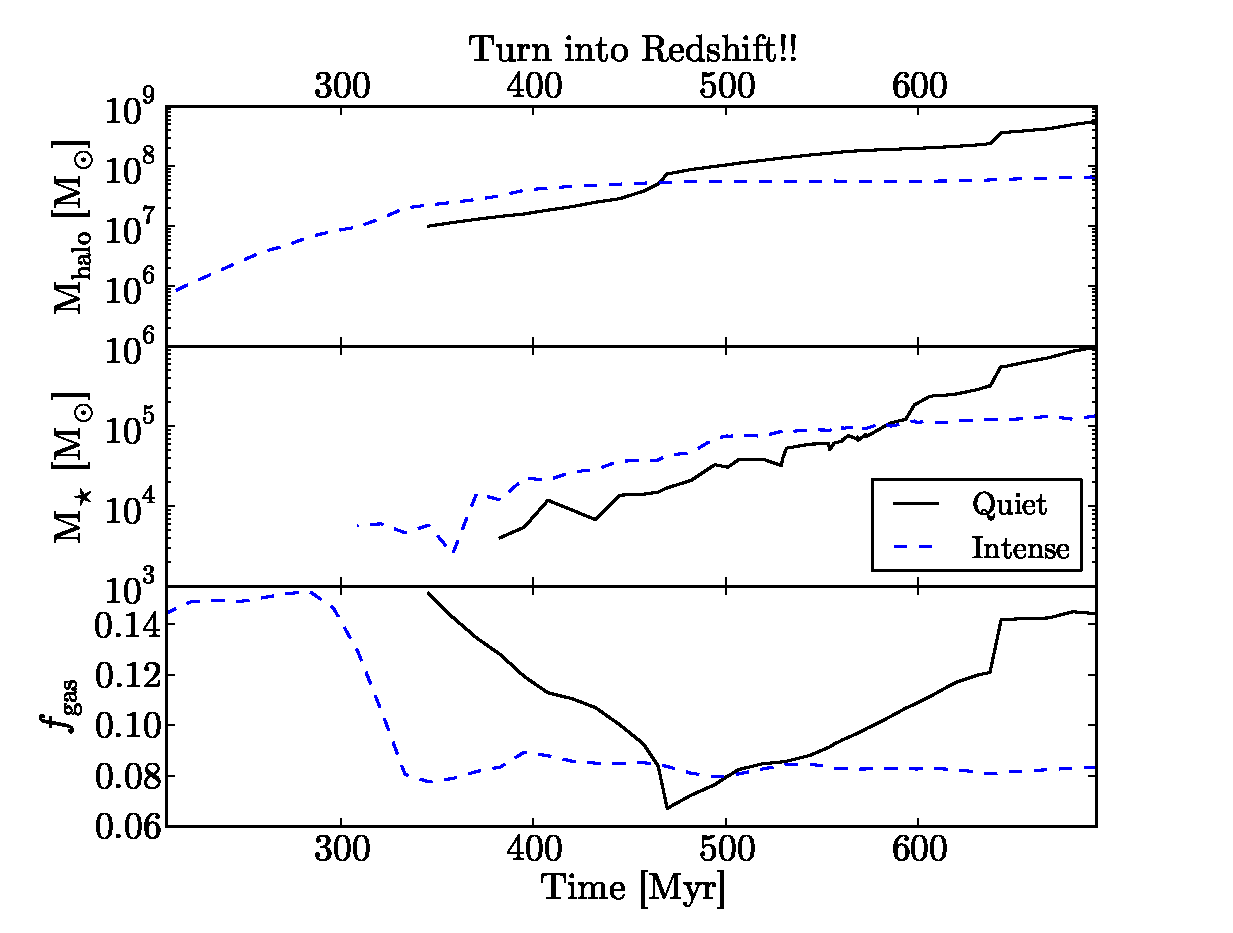
\includegraphics[width=\textwidth]{f1.eps}
\caption{\label{fig:projections} Density-weighted projections of gas
  density (top), temperature (middle), and metallicity (bottom) at
  $z=7$.  The left column shows the entire simulation volume, where
  the center and right columns focus on the intense and quiet halos,
  which are marked by left and right arrows in the upper-left panel.
  The metallicity projections are a composite picture of metals
  originating from Pop III (red) and Pop II (blue) stars with magenta
  indicating a mixture of the two.}
\end{figure*}

\clearpage
\begin{figure*}
% Need to include f2.eps
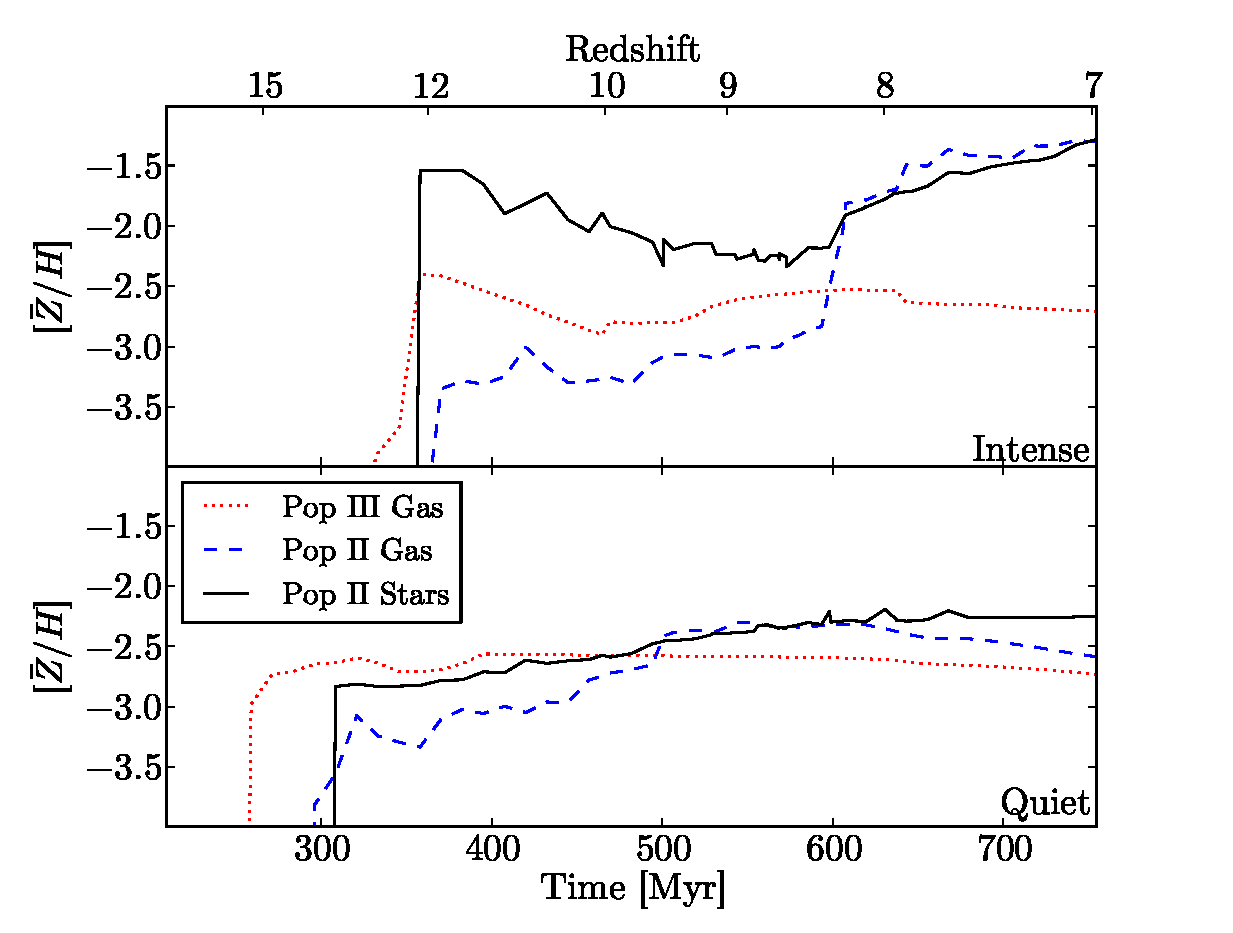
\includegraphics[width=\textwidth]{f2.eps}
\caption{\label{fig:evo} (a) Evolution of the total halo mass (top),
  stellar mass (middle), and gas fraction (bottom) of the quiet
  (dashed) and intense (solid) halos.  (b) Mass-weighted stellar
  metallicities and gas metallicities enriched by Pop II and Pop III
  SNe of the intense (top) and quiet (bottom) halos.}
\end{figure*}

\clearpage
\begin{figure*}
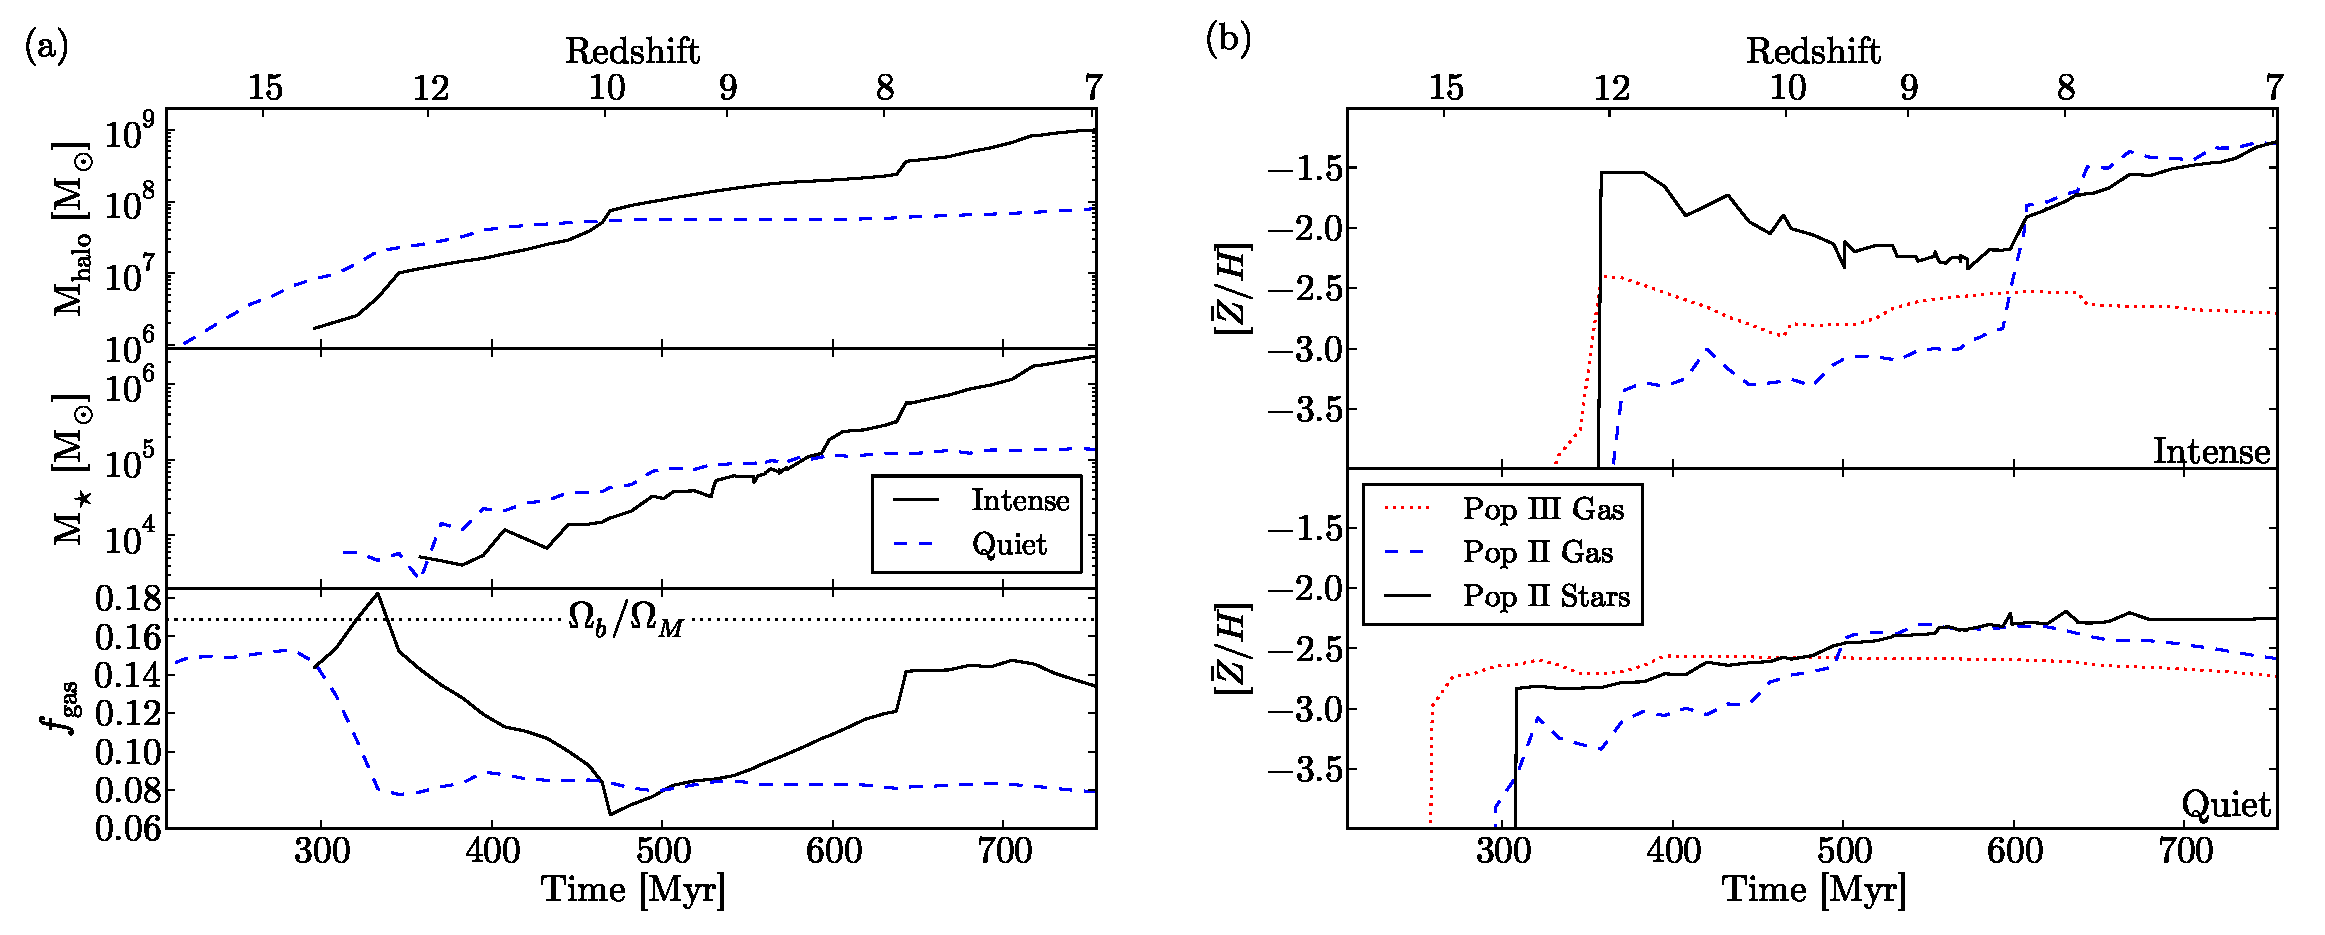
\includegraphics[width=\textwidth]{f3.eps}
\caption{\label{fig:pops} The scatter plots show the SF history of the
  quiet (left) and intense (right) halos as a function of metallicity
  at $z=7$.  Each circle represents a star cluster, whose area is
  proportional to its mass.  The open circles in the upper right
  represent sizes of $10^3$, $10^4$, and $10^5$ \Ms~star clusters.
  The dashed lines in the right panel guide the eye to two stellar
  populations that were formed in two satellite halos, merging at
  $z=7.5$.  The upper histogram shows the SF rate.  The right
  histogram depicts the stellar metallicity distribution.}
\end{figure*}

%\noindent {\bf Fig. 1.} Please do not use figure environments to set
%up your figures in the final (post-peer-review) draft, do not include graphics in your
%source code, and do not cite figures in the text using \LaTeX\
%\verb+\ref+ commands.  Instead, simply refer to the figure numbers in
%the text per {\it Science\/} style, and include the list of captions at
%the end of the document, coded as ordinary paragraphs as shown in the
%\texttt{scifile.tex} template file.  Your actual figure files should
%be submitted separately.

%\include{som}

\end{document}
